%%%%%%%%%%%%%%%%%%%%%%%%%%%%%%%%%%%%%%%%%%%%%%%%%%%%%%%%%%%%%%%%%%%%%%
%%                     delay
%%%%%%%%%%%%%%%%%%%%%%%%%%%%%%%%%%%%%%%%%%%%%%%%%%%%%%%%%%%%%%%%%%%%%%

\subsection{Glyph: \glyph{delay}}\label{sec:delay}

The glyph \glyph{delay} is used to denote that the \glyph{activity node} linked as input does not produce the influence immediately.

\begin{glyphDescription}
 \glyphSboTerm SBO:0000225 ! delay.
 \glyphOrigin One \glyph{biological activity} (\sect{af:biologicalActivity}) via a \glyph{logical arc} (\sect{af:logicArc}).
 \glyphTarget A \glyph{modulation arc} (\sect{af:ANs}) other than \glyph{equivalence arc}.
 \glyphContainer \glyph{Delay} is represented by a circle, with two connectors located at the opposite side for inputs and output.
 \glyphLabel \glyph{Delay} is identified by the greek letter ``$\tau$`` (``TAU'') placed in an unbordered box attached to the center of the node.
 \glyphAux \glyph{Delay} does not carry any auxiliary items.
\end{glyphDescription}

\begin{figure}[H]
  \centering
  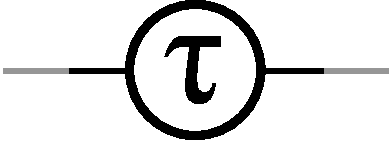
\includegraphics[scale = 0.5]{images/build/delay.pdf}
  \caption{The \AF glyph for \glyph{delay}.}
  \label{fig:delay}
\end{figure}
\normalcolor
